In this chapter, we define the actual event detection algorithm. First, we describe the original method used by \cite{event-detection}. Then, we make a change to incorporate semantic similarity through the word embeddings obtained in \autoref{chap:data-preprocessing}. Finally, we introduce an alternative algorithm that depends on word clustering using a custom distance function.

The original algorithm creates events as sets of related keywords by greedily minimizing a cost function combining temporal and semantical distance between words. However, the paper used only a simple notion of semantical distance, namely the document overlap between words. This demands that there exists at least one document containing all the words used to represent an event. This is a strong requirement, since the documents may use different vocabularies while conveying similar information.  As a result, the events are split into multiple keyword sets, leading to redundancy.

In an attempt to solve this problem, we modify the cost function, replacing the document overlap by Word2Vec-based similarity. This does not require the words to appear in exactly the same documents, only that they have similar semantics. We refer to this method as \textit{greedy approach}.

Realizing that the task of constructing keyword sets resembles the task of word clustering, we propose an alternative algorithm. Here, we apply a clustering algorithm to the words, using a modification of the cost function as a distance measure. This is a method referred to as \textit{cluster-based approach}.

First, we briefly describe the original method for reference. This will make it clear which parts of the function we modify. It will also allow us to make reference to the original method in \autoref{chap:evaluation}, where we compare all three algorithms.

\section{Original method}
As stated in the introduction, the original method performs greedy minimization of a cost function defined over sets of words. The cost function consists of trajectory distance measuring the word distance in temporal domain, and document overlap, standing for distance in the semantic domain. We first describe these two components and then combine them into the cost function.

\subsection{Trajectory distance}
Before measuring the trajectory distance, the trajectories are smoothened by fitting a probability density function to them. We adapt a similar technique in \autoref{chap:document-retrieval} where it is described in more detail. Our event detection modifications do not use the original smoothing though, and we refer the reader to the original paper for more details.

After normalization to unit sum, the (smoothened) trajectory $\vect{\trajn}_{w}$ of a word $w$ can be interpreted as a probability distribution over the stream days. The element $\trajn_{w}(i)$ then denotes the probability that $w$ appears on day $i$. This interpretation allows to compare the trajectories using information-theoretic techniques, notably the information divergence \citep{information-theory}.

In the original paper, the authors first defined the distance between trajectories of two words $v$ and $w$ as $\trajdist{\vect{\trajn}_{v}}{\vect{\trajn}_{w}} = \max \left\{ \kl{\vect{\trajn}_{v}}{\vect{\trajn}_{w}}, \kl{\vect{\trajn}_{w}}{\vect{\trajn}_{v}} \right\}$, symmetrizing the Kullback-Leibler divergence KL \citep{kl-divergence}.

Then, the distance is generalized to a whole set of words $\featset$ as

\begin{equation} \label{eq:trajectory-distance}
	\text{Dist}( \featset ) = \max_{v, w \in \featset} \trajdist{\vect{\trajn}_{v}}{\vect{\trajn}_{w}}.
\end{equation}

\subsection{Document overlap}
The document overlap is again first defined for a pair of words $v$ and $w$ as $\text{DO}\left( v, w \right) = \frac{| \featset_{v} \cap \featset_{w} |}{\min \left\{ | \featset_{v} |, | \featset_{w} | \right\}}$, where $\featset_{j} = \{ i \mid \bowmat_{ij} = 1 \}$ is the set of all documents containing the word $j$. The higher the document overlap, the more documents do the two words have in common, which makes them more likely to be correlated.

The overlap is again generalized to a set of words $\featset$ as

\begin{equation} \label{eq:document-overlap}
	\text{DO}( \featset ) = \min_{v, w \in \featset} \text{DO}( v, w ).
\end{equation}

\subsection{Cost function}
The cost function is a combination of the trajectory distance and document overlap of a set of words. It is defined as

\begin{equation} \label{eq:cost-function-original}
	\text{C}( \featset ) = \frac{\text{Dist}( \featset )}{\text{DO}( \featset ) \cdot \sum_{w \in \featset} \text{DPS}_{w}}.
\end{equation}

Since the algorithm attempts to minimize it, the intuitive result is a set of words with low trajectory distance and high document overlap. The algorithm will also prefer words of higher importance due to the last term of the denominator, counting in the power spectra.

\newpage

\subsection{Event detection algorithm}
The algorithm, called \textit{unsupervised greedy event detection algorithm} in the original paper, is defined as follows.

\begin{algorithm}[H]
\begin{algorithmic}[1]
\caption{Unsupervised greedy event detection}
\label{alg:greedy-event-detection}
\Input $\text{Word set} ~ \text{EW obtained in \autoref{chap:word-analysis}, matrices } \bowmat \text{ and }\trajmat \text{, word DPS}$

\State $\text{Sort the words in descending DPS order: } \text{DPS}_{w_{1}} \geq \dots \geq \text{DPS}_{w_{\left\vert \text{EW} \right\vert}}$

\State $k = 0$

\ForEach{$w \in \text{EW}$}
	\State $k = k + 1$	
	\State $e_{k} = \{ w \}$
	\State $cost_{e_{k}} = \frac{1}{DPS_{w}}$
	\State $\text{EW} = \text{EW} \setminus w$
	
	\While{$\text{EW} \neq \emptyset$}
		\State $m = \argmin\limits_{m}{\text{C}( e_{k} \cup w_{m} )}$

		\If{$\text{C}( e_{k} \cup w_{m} ) < cost_{e_{k}}$}
			\State $cost_{e_{k}} = \text{C}( e_{k} \cup w_{m} )$
			\State $e_{k} = e_{k} \cup w_{m}$
			\State $\text{EW} = \text{EW} \setminus w_{m}$
		\Else
			\Break
		\EndIf
	\EndWhile
\EndFor

\Output $\text{Events} ~ \{ e_{1}, \dots, e_{k} \}$
\end{algorithmic}
\end{algorithm}

The algorithm works by greedily minimizing the cost function \eqref{eq:cost-function-original}. Once it is minimized, an event is produced, consisting of all the words found since last event.

The words are sorted in descending DPS order before entering the minimization loop, so that the most important words are processed first. This assures that the most eventful words are assigned together, without wasting them to appear with low quality words.

\cite{event-detection} did not provide the time complexity of the algorithm, which we attempt to estimate now. The execution time is dominated by the main loop on lines 3 through 18. The outer loop must execute $\mathcal{O}(|\text{EW}|)$ times. In each of the iterations, the inner loop is executed at most $|\text{EW}|$ times, making it $\mathcal{O}(|\text{EW}|)$ as well. The argmin statement on line 9 must search through the whole remaining $|\text{EW}|$ words, also making it run $\mathcal{O}(|\text{EW}|)$ times.

If the number of eventful words is low enough, the pairwise trajectory distance and document overlap can be precomputed. This makes the cost function take $\mathcal{O}(|\text{M}|^{2})$ time when applied to a set M. If the distances are not precomputed, the cost function execution requires $\mathcal{O}(|\text{M}|^{3})$ time.

We were unable to precisely determine the cost function's complexity with respect to the set EW, as it is always applied on the currently composed event. However, during our experiments, the number of words comprising an event never exceeded 10 in the original method. This makes the cost function's asymptotic complexity negligible compared to the main loop.

The resulting complexity of the algorithm is therefore $\mathcal{O}(|\text{EW}|^{3} \cdot c)$, where $c$ is the complexity of the cost function.


\begin{figure}[H]
  \centering
  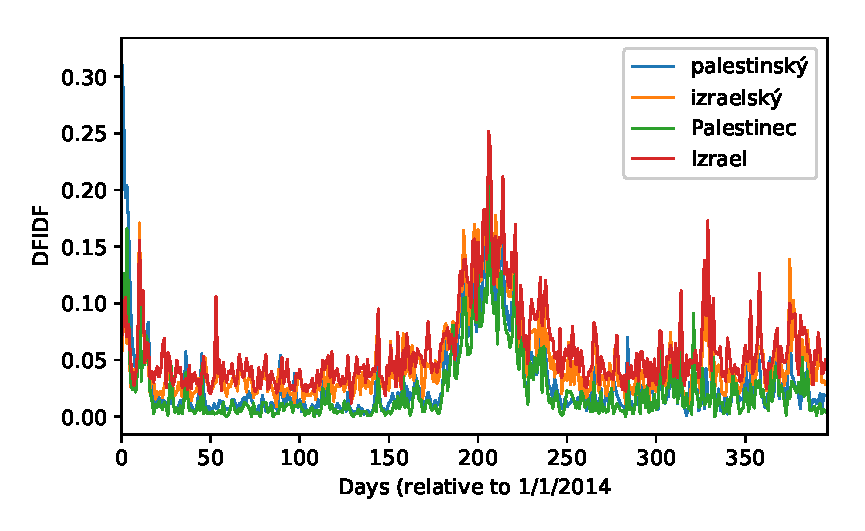
\includegraphics{original_event}  % original event
  \caption{Example of an event detected using the original method. The event consists of the words \textit{palestinian}, \textit{israeli}, \textit{Palestinian} and \textit{Israel}, respectively.}
  \label{fig:original-event}
\end{figure}


\section{Greedy approach}
In this section, we modify the original method to use the Word2Vec model to measure semantic similarity between words. Unlike the document overlap \eqref{eq:document-overlap}, this new similarity measure is able to distinguish semantically similar words even when they do not appear in the same documents. This may happen, for instance, when different authors each use distinct vocabulary when referring to the same event.


\subsection{Semantic similarity}
Some of the astounding results of the Word2Vec model arise from semantically similar words forming clusters \citep{linguistic-regularities} in terms of cosine similarity, which is a standard measure used in information retrieval \citep{information-retrieval, cosine-similarity}.

We replace the document overlap in the cost function \eqref{eq:cost-function-original} by cosine similarity between Word2Vec embeddings, though with a small modification. The cosine similarity is bounded in $[-1, 1]$ with -1 denoting the least degree of similarity. This means that the cost function would reach negative values for highly dissimilar words. This would be a problem, as Algorithm \ref{alg:greedy-event-detection} attempts to minimize it. Consequently, we will transform the cosine similarity into $[0, 1]$, just like the document overlap \eqref{eq:document-overlap}.

The similarity between a set of words $\featset$ and a word $w \notin \featset$ is defined as

\begin{equation}
	\semsim{\featset}{w} = \left( \frac{\inp[\big]{\bar{\embed}_{\featset}}{\embed_{w}}}{\| \bar{\embed}_{\featset} \| \cdot \| \embed_{w} \|} + 1 \right) /\ 2,
\end{equation}

where $\bar{\embed}_{\featset}$ is the mean of all vector embeddings of $\featset$ and $\embed_{w}$ is the vector embedding of $w$. Here, the mean vector virtually represents the central topic of words in $\featset$.


\subsection{Cost function}
We redefine the cost function \eqref{eq:cost-function-original} as

\begin{equation} \label{eq:cost-function}
	\cost{\featset}{w} = \frac{\text{Dist}( \featset \cup w )}{\semsim{\featset}{w} \cdot \sum_{u \in \featset \cup w}{\text{DPS}_{u}}},
\end{equation}

where $\text{Dist}(\cdot)$ is the original trajectory distance function \eqref{eq:trajectory-distance}.

In the original method, \cite{event-detection} defined the cost function \eqref{eq:cost-function-original} for a set of words. However, in Algorithm \ref{alg:greedy-event-detection}, it is always applied on a union of an event constructed so far, and a newly added word. The new cost function must now be applied on such event and word separately due to the nature of Word2Vec similarity definition.

Having constructed the cost function, we use Algorithm \ref{alg:greedy-event-detection} to detect events once again.


\begin{figure}[H]
  \centering
  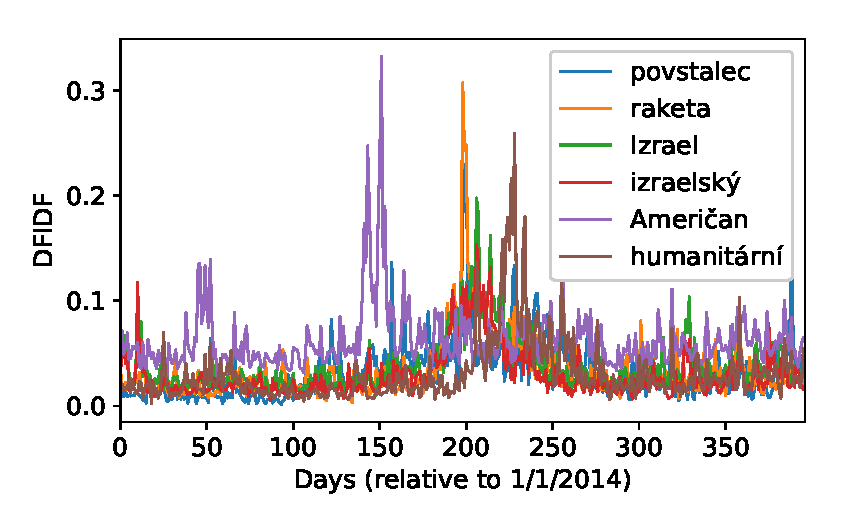
\includegraphics{greedy_event}  % greedy event
  \caption{Example of an event detected using the greedy method. The event consists of the words \textit{to shoot}, \textit{missile}, \textit{Israel} and \textit{israeli}, and is related to the same real event as \autoref{fig:original-event}.}
  \label{fig:greedy-event}
\end{figure}


\section{Cluster-based approach}
Realizing that the keyword-based event detection resembles word clustering, we decided to investigate this idea. In the final method, we apply a clustering algorithm equipped with a custom distance function to the set of eventful words. The distance function is actually a modification of the cost function yet again, though some means have to be taken to make it usable in this context. First, we need to consider a proper clustering algorithm.

The obvious requirement for the clustering algorithm is that it must require no prior knowledge of the desired number of clusters. Another requirement is that the algorithm must accept a custom distance measure.

We considered three candidate algorithms: Affinity propagation \citep{affinity-propagation}, DBSCAN \citep{dbscan} and its modification, HDBSCAN \citep{hdbscan}.

During our experimentation, Affinity propagation performed poorly, its clusters being often seemingly random and of low quality. The quality of HDBSCAN clusters was considerably better, though the algorithm took longer to converge as the number of eventful words grew. It also required to tune multiple parameters, which was difficult to do without any annotated data. We decided to use the DBSCAN algorithm, which outperformed Affinity propagation as well, and does not require to tune as many parameters as HDBSCAN.

In addition to the previously stated requirements, DBSCAN is also capable of filtering out noisy samples (in our case words), not fit for any of the clusters. This property will prove advantageous for our task, as will become clear during the evaluation in \autoref{sec:noise-evaluation}.


\subsection{Noise filtering}
Before we apply clustering, we filter out the noisy parts from the word trajectories. Most words are on some level reported all the time, though only a fraction of these reportings corresponds to notable events. Unlike the greedy optimization described previously, clustering is prone to such noise, and would yield clusters of poor quality, often with trajectories being put together only due to their noisy parts being similar. Additionaly, with DBSCAN capable of filtering out noisy samples, some high quality words could be discarded precisely due to this noise in their (otherwise eventful) trajectories.

We want to keep only those trajectory parts exceeding a certain frequency level, distinguishing notable bursts from the general noise. We do this by computing a cutoff value for each event trajectory and discarding the sectors falling under this cutoff. This procedure is adopted from \cite{online-search-queries}. The algorithm is based on computing a moving average along the trajectory, and works as follows:

\begin{algorithm}[H]
\begin{algorithmic}[1]
\caption{Burst filtering}
\label{alg:burst-filtering}
\Input $\text{window-length} \ l,\ \text{word trajectory} \ \vect{\traj_{w}}$

\State $\vect{MA}_{l} = \text{Moving Average of length} ~ l ~ \text{for} ~ \vect{\traj}_{w} = \left[ \traj_{w}(1), \traj_{w}(2), \dots, \traj_{w}(\streamlen) \right]$

\State $\mathit{cutoff} = \text{mean} \left( \vect{MA}_{l} \right) + \text{std} \left( \vect{MA}_{l} \right)$

\State $\vect{bursts}_{w} = \left[ \traj_{w}(t) \mid \traj_{w	}(t) > \mathit{cutoff} \right]$

\Output $\vect{bursts}_{w}$
\end{algorithmic}
\end{algorithm}


\subsection{Distance function}
We now define the distance function used by DBSCAN. It conveys similar information as the cost function in the previous two algorithms. We still need to measure the trajectory distance as well as semantic similarity between words, though the distance will now be defined strictly pairwise.

For a measure of trajectory distance, we replace the Kullback-Leibler divergence by the Jensen-Shannon divergence JSD \citep{js-divergence-1}, which is symmetric in its arguments. This is a necessary property of the distance function.

Although \cite{event-detection} did symmetrize the Kullback-Leibler divergence, they did not provide any source for their symmetrization form. We were unable to find a case where that particular form was used, though we discovered the Jensen-Shannon divergence, which comes from stronger mathematical background \citep{js-divergence-1, js-divergence-2}. It also tended to improve the clustering quality during our experimentation, as opposed to the original symmetrization. We then decided to replace the original paper's KL-divergence symmetrization by the JS-divergence.

Instead of semantic \textit{similarity}, we measure semantic \textit{distance} as the Euclidean distance between two word vector embeddings. The reason is that Euclidean distance is unbounded, which makes it possible for the samples to be spread farther apart. Since DBSCAN is a density-based clustering algorithm, having high density areas consisting of words with low trajectory distance and similar cosine similarities would cause them to appear in the same cluster. This would cluster the words only in terms of their trajectories, not semantics.

The distance between two words $v$ and $w$ with (normalized and filtered using Algorithm \ref{alg:burst-filtering}) trajectories $\vect{\trajn}_{v},\ \vect{\trajn}_{w}$ and Word2Vec embeddings $\embed_{v},\ \embed_{w}$ is now defined as

\begin{equation}
	\distfunc{v}{w} = \jsd{\vect{\trajn}_{v}}{\vect{\trajn}_{w}} \cdot \| \embed_{v} - \embed_{w}\|_{2},
\end{equation}

with $\jsd{\vect{p}}{\vect{q}} = \frac{1}{2} \left( \kl{\vect{p}}{\vect{m}} + \kl{\vect{q}}{\vect{m}} \right) ,\ \vect{m} = \frac{1}{2} \left( \vect{p} + \vect{q} \right)$.


\subsection{Event detection}
Now, we describe the cluster-based event detection algorithm, which is a direct application of the DBSCAN algorithm and consequent noise filtering.

\begin{algorithm}[H]
\begin{algorithmic}[1]
\caption{Cluster-based event detection}
\Input $\text{Word set EW obtained in \autoref{chap:word-analysis}, matrix } \trajmat \text{, word embeddings for EW}$

\State Precompute a distance matrix $\distmat \in \R^{\left\vert \text{EW} \right\vert \times \left\vert \text{EW} \right\vert}$ with $\distmat_{ij} = \distfunc{w_{i}}{w_{j}}$

\State Apply DBSCAN to $\distmat$, obtaining $k$ clusters and the noisy cluster

\ForEach{$(w, cluster) \in \text{DBSCAN.clusters}$}
	\If{$cluster \neq noise$}
		\State $e_{cluster} = e_{cluster} \cup w$
	\EndIf
\EndFor

\Output $\text{Events} ~ \{ e_{1}, e_{2}, \dots, e_{k} \}$
\end{algorithmic}
\end{algorithm}


\begin{figure}[H]
  \centering
  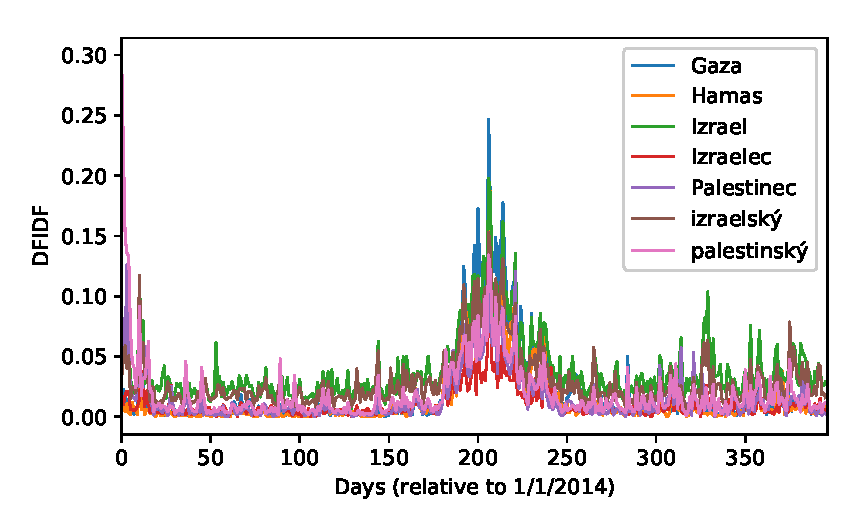
\includegraphics{cluster_event}  % cluster event
  \caption{Example of an event detected using the cluster-based method. The event is related to the same real event as \autoref{fig:original-event} and \autoref{fig:greedy-event}. Note that the trajectories are clear of noise due to application of Algorithm \ref{alg:burst-filtering}}
  \label{fig:cluster-event}
\end{figure}
